\section{\bt{Evaluation}{实验评估}}
\label{sec:evaluation}
\subsection{\bt{Experimental setup}{实验设置}}
\label{sec:experimental-setup}
\label{sec:metric-setup}
\bi{\emph{Workloads.} RelBench v1~\cite{robinson2024relbench} supplies six classification/regression tasks on rel-stack/rel-trial (Table~\ref{tab:relbench}). Five cutoffs, 91/365 days apart, append data and restart conversations; the last matches the official split. A separate official-API cohort uses the first three cutoffs, with policy tuning on rel-amazon/user-churn outside the evaluation databases. Analytical studies use TPC-DS SF1~\cite{tpcds2026benchmark} (24 tables, 2.9M store-sales rows), synthetic retail (1M sales, 396k returns, 500k catalog sales), and TPC-H SF1~\cite{tpch2026benchmark}. Five metrics each provide two learning questions and five scored forms spanning new periods, differences, and monthly comparisons. Replay extends to SSB~\cite{oneil2009ssb} and BIRD financial~\cite{li2023bird}.}
{\emph{负载。}RelBench v1~\cite{robinson2024relbench}提供 rel-stack／rel-trial 六项分类／回归任务（表~\ref{tab:relbench}）。五截点间隔 91／365 天，追加数据并重启对话，末截点匹配官方划分。独立官方 API 批次使用前三截点，策略在评估库之外的 rel-amazon/user-churn 调优。分析实验使用 TPC-DS SF1~\cite{tpcds2026benchmark}（24 表、290 万行门店销售）、合成零售（100 万行销售、39.6 万行退货、50 万行目录销售）与 TPC-H SF1~\cite{tpch2026benchmark}；五指标各有两道学习题及五种跨期间、差值和月度比较计分题。回放另覆盖 SSB~\cite{oneil2009ssb} 和 BIRD financial~\cite{li2023bird}。}
\label{sec:setup-baselines}
\bi{\emph{Methods.} Predictive agents share tools and validation feedback without test-label access. ACE~\cite{zhang2026ace} uses released no-ground-truth Reflector/Curator prompts, one update/session, and an 80k-token playbook per task agent. AWM~\cite{wang2025awm} retains online workflow induction and private agent/database scope, adapting web actions to SQL with a separate rel-f1 demonstration. G-Memory~\cite{zhang2025gmemory} retains its released hierarchical store, shared per database; MiniLM and LLM scoring retrieve one trajectory and up to five insights. DeepPrep~\cite{fan2026deepprep} retains released prompts, reasoning, 31 operators, and rule execution (five exploration turns, 50 operators/chain, 2,000 training seeds), restarting at every task/cutoff. FeatPilot*~\cite{liang2025featpilot} retains join-path search, quality pruning, importance-times-quality ranking, and redundancy control (ten features, heap 30, threshold 0.1); training-sample quality, common-learner importance, and text length replace its learned quality estimator, AutoGluon, and embeddings. SQL enforces seed-time bounds.}
{\emph{方法。}预测智能体共用工具和验证反馈，不接触测试标签。ACE~\cite{zhang2026ace}使用发布的不依赖真实答案的反思／整理提示词，每会话更新一次，每任务智能体保留 80k-token 手册。AWM~\cite{wang2025awm}保留在线工作流归纳及私有智能体／数据库作用域，以 SQL 适配网页动作，示例来自独立 rel-f1。G-Memory~\cite{zhang2025gmemory}保留发布的分层存储，在库内共享，通过 MiniLM 和 LLM 评分检索一条轨迹及最多五条洞见。DeepPrep~\cite{fan2026deepprep}保留发布的提示词、推理、31 算子与规则执行（五轮探索、每链 50 算子、2,000 训练种子），每任务／截点重启。FeatPilot*~\cite{liang2025featpilot}保留连接路径搜索、质量剪枝、重要性与质量乘积排序及冗余控制（十特征、候选堆 30、阈值 0.1），以训练样本质量、共同学习器重要性、文本长度替代学习型质量估计器、AutoGluon 和嵌入，SQL 施加种子时间界限。}
\bi{Figure~\ref{fig:twoschemas} compares SQL-adapted ACE/AWM, official G-Memory, and full \system{} on three metrics/schema, two learning questions/metric, and \PubDistinctQuestions{} distinct scored questions. Six unchanged baseline cells reuse frozen corrected runs; the repaired system reruns the original bank. A new agent B receives the same business definition and three spending-fixed M3 forms: period difference, highest month, and largest monthly increase. Conversations restart; changes restore post-held-out memory. All methods receive the same format of their last three own results and binary correctness, without reference answers/SQL, and retain normal memory updates. Native lookups are capped at three/question; validation caching keys SQL/dependency versions without caching results.}
{图~\ref{fig:twoschemas}比较 SQL 适配的 ACE／AWM、官方 G-Memory 与完整 \system{}，每模式三指标、各两道学习题，共 \PubDistinctQuestions{} 道不同计分问题。六个未变更的基线格复用已冻结的修复后运行，修复后的系统重跑原题库。新智能体 B 获得相同业务定义及仅按预算固定的三种 M3 题型：期间差值、最高月份、最大月度增幅。每题重启对话，各变化恢复留出后的记忆。所有方法按同一格式接收自身近三题结果及二值正确性，不接收参考答案／SQL，并保留正常记忆更新。原生查找每题限三次；验证缓存按 SQL／依赖版本索引，不缓存结果。}
\bi{\emph{Execution.} Hardware provides 48 vCPUs, 98\,GiB RAM, and PostgreSQL 18.6. Predictive agents use \code{deepseek-flash} (\llmmodel{}), thinking at low effort; analytical agents/extraction use high effort, 20 turns, and a 60\,s SQL limit (120\,s for TPC-DS/TPC-H). Figure~\ref{fig:twoschemas} uses low effort and 120\,s SQL limits. AWM/G-Memory memory calls are non-thinking, capped at 2,048/512 output tokens. Common LightGBM 4.6.0~\cite{ke2017lightgbm} uses 50k training rows (seed 42), 300 trees, learning rate 0.05, and 63 leaves. SQL returns one row/seed and at most 100 features within 600\,s; future-hidden audits recompute up to 5,000 seeds. Five-/three-cutoff budgets are 40/24 planner calls and eight/five validations; stop after two non-improving validations. Refitting the prior solution permits one further improvement within five/three calls.}
{\emph{执行。}硬件为 48 vCPU、98\,GiB 内存及 PostgreSQL 18.6。预测智能体使用 \code{deepseek-flash}（\llmmodel{}），low 思考强度；分析智能体／提炼为 high 强度、20 轮，SQL 限时 60 秒（TPC-DS／TPC-H 为 120 秒）。图~\ref{fig:twoschemas}统一使用 low 强度和 120 秒 SQL 限时。AWM／G-Memory 记忆调用关闭思考，输出上限 2,048／512 token。共同 LightGBM 4.6.0~\cite{ke2017lightgbm}使用 50k 训练行（种子 42）、300 树、学习率 0.05、63 叶子。SQL 每种子一行、最多 100 特征、限时 600 秒；隐藏未来数据的审计重算最多 5,000 种子。五／三截点预算为 40／24 次规划、八／五次验证，连续两次未改进即停止；达到前一方案重训分数后，允许在五／三次调用内再改进一次。}
\label{sec:setup-metrics}
\bi{\emph{Metrics.} Quality margins are an AUC decrease $\leq0.01$ or MAE increase $\leq2\%$ relative to no memory. Invalid/leaking solutions retain cost and use entity-reference scores; valid counts exclude fallback. Analytical references run after truth updates and before representation changes. Tokens include memory updates; reuse excludes cutoff 1. Agent-call counts exclude internal memory calls. Shared-server session times include API waits and online database work, excluding leakage audits and post-session publication; maintenance includes metadata SQL. RelBench cutoffs are dependent observations, not repetitions.}
{\emph{计量。}相对无记忆的质量门槛为 AUC 下降 $\leq0.01$ 或 MAE 增加 $\leq2\%$。无效／泄漏方案保留成本、回退实体参照分数，有效数不含回退。分析参照在事实更新后、表示变化前执行。token 包括记忆更新，复用不含首截点，智能体调用不含内部记忆调用。共享服务器会话时间含 API 等待及在线数据库工作，不含泄漏审计与会话后发布；维护含元数据 SQL。RelBench 截点是相关观测，不是独立重复。}
\subsection{\bt{Predictive reuse}{预测任务复用}}
\label{sec:relbench-eval}
\begin{table*}[t]
\caption{\bt{RelBench: predictive quality, valid solutions, and reuse cost. Each method runs three tasks at five cutoffs per database.}{RelBench：预测质量、有效方案与复用代价。每种方法在每个数据库上运行三个任务、五个截点。}}
\label{tab:relbench}
\centering
\ifbilingual\footnotesize\else\small\fi
\setlength{\tabcolsep}{2.8pt}
\renewcommand{\arraystretch}{1.08}
\newcommand{\RbPanelHeader}[4]{%
  \multicolumn{12}{@{}l}{\textbf{#1}}\\[2pt]
  & \multicolumn{6}{c}{\bh{Reuse cost: cutoffs 2--5}{复用代价：截点 2--5}}
  & \multicolumn{3}{c}{\bh{Mean test score: cutoffs 1--5}{平均测试分数：截点 1--5}}
  & \multicolumn{2}{c}{\bh{Quality summary}{质量汇总}}\\
  \cmidrule(lr){2-7}\cmidrule(lr){8-10}\cmidrule(l){11-12}
  \bh{Method}{方法} & \bh{Tokens\\(M)}{token\\（百万）} & \bh{Token\\ratio}{token\\比率}
  & \bh{LLM\\calls}{LLM\\调用} & \bh{Tool\\calls}{工具\\调用}
  & \bh{Obs.\\min}{观测\\分钟} & \bh{Cost\\(USD)}{美元}
  & #2 & #3 & #4 & \bh{Valid\\sessions}{有效会话} & \bh{Quality\\tasks}{达标任务}\\
  \midrule
}
\begin{tabular*}{\textwidth}{@{\extracolsep{\fill}}lrrrrrrrrrcc@{}}
\toprule
\RbTableBody
\bottomrule
\end{tabular*}
\par\smallskip
\parbox{\textwidth}{\footnotesize\raggedright
\bt{Cost columns total 12 sessions at cutoffs 2--5, including memory operations; token ratios are relative to no memory. Test scores average all five cutoffs, using the entity-table reference for sessions without a valid solution. \emph{Valid sessions}: non-fallback solutions (/15). \emph{Quality tasks}: tasks retaining no-memory predictive quality (/3), with $\mathrm{AUC}\geq\mathrm{AUC}_0-0.01$ or $\mathrm{MAE}\leq 1.02\,\mathrm{MAE}_0$. Subscript 0 denotes no memory; best task means are bold. Time and USD accounting are specified in Section~\ref{sec:relbench-eval}.}{代价列合计截点 2--5 的 12 个会话，含记忆操作；token 比率以无记忆为参照。测试分数取五个截点的平均，无有效方案的会话采用实体表参照分数。有效会话计数排除参照回退（共 15 个）；达标任务指保持无记忆预测质量的任务数（共 3 项），满足 $\mathrm{AUC}\geq\mathrm{AUC}_0-0.01$ 或 $\mathrm{MAE}\leq 1.02\,\mathrm{MAE}_0$。下标 0 表示无记忆；各任务最佳平均分加粗。时间与美元计量见第~\ref{sec:relbench-eval} 节。}
}
\end{table*}

\begin{figure}[t]
\centering
% Vector drawing generated by tools/figures/relbench_cumulative.py from exp/2026-10-20-relbench/paper-sessions.json; rerun it after the numbers change.
\ifbilingual
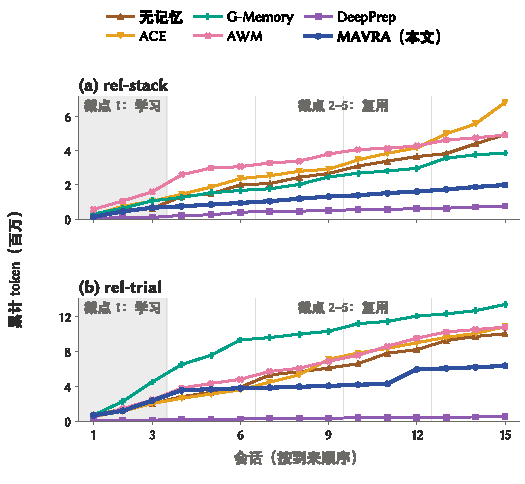
\includegraphics[width=\linewidth]{figures/relbench-cumulative-zh}
\else
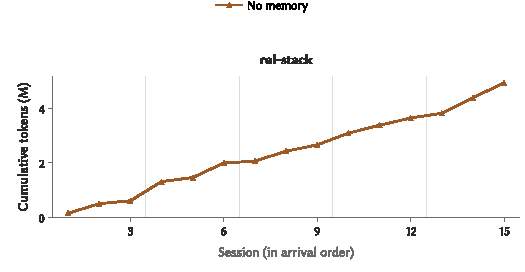
\includegraphics[width=\linewidth]{figures/relbench-cumulative}
\fi
\caption{\bt{Cumulative tokens of the RelBench sessions in arrival order, memory operations included; thin rules separate the five cutoffs. After the first cutoff, \system's agents start from the verified task program and its curve flattens, while the other methods keep paying for exploration at every cutoff.}{按到来顺序累计的 RelBench 会话 token（含记忆操作）；细线分隔 5 个截点。第一个截点之后，\system\ 的智能体从经验证的任务方案出发，曲线变平；其他方法在每个截点都继续为探索付费。}}
\label{fig:relbench-cumulative}
\Description{Two line charts, rel-stack and rel-trial, of cumulative tokens in millions against the session index from 1 to 15, one line per method.}
\end{figure}

\bi{Table~\ref{tab:relbench} compares seven methods over six tasks and five cutoffs (210 sessions). All six \system{} task means meet the quality margins. Relative to no memory, reuse-stage tokens fall by \RbStackMavraTokSave\%/\RbTrialMavraTokSave\% on rel-stack/rel-trial; including learning and memory operations, savings are \RbStackMavraTokSaveAll\%/\RbTrialMavraTokSaveAll\%. Figure~\ref{fig:relbench-cumulative} plots the six LLM-based methods; non-LLM FeatPilot* remains in the table. USD estimates use historical per-million-token rates of \$0.003 cached input, \$0.15 uncached input, and \$0.60 output.}
{表~\ref{tab:relbench}比较七种方法、六项任务与五截点（210 会话）。\system{} 六项任务均值均达到质量门槛；相对无记忆，rel-stack／rel-trial 的复用 token 减少 \RbStackMavraTokSave\%／\RbTrialMavraTokSave\%，计入学习与记忆操作后减少 \RbStackMavraTokSaveAll\%／\RbTrialMavraTokSaveAll\%。图~\ref{fig:relbench-cumulative}展示六种 LLM 方法，非 LLM 的 FeatPilot* 保留在表中。美元估价沿用历史每百万 token 的缓存输入 0.003、未缓存输入 0.15、输出 0.60 美元。}
\label{sec:sharing-eval}
\begin{figure}[t]
\centering
\ifbilingual
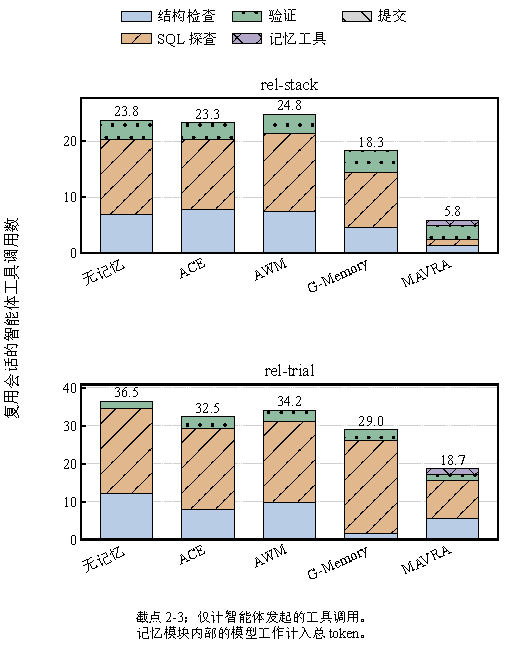
\includegraphics[width=\linewidth]{figures/reuse-work-zh}
\else
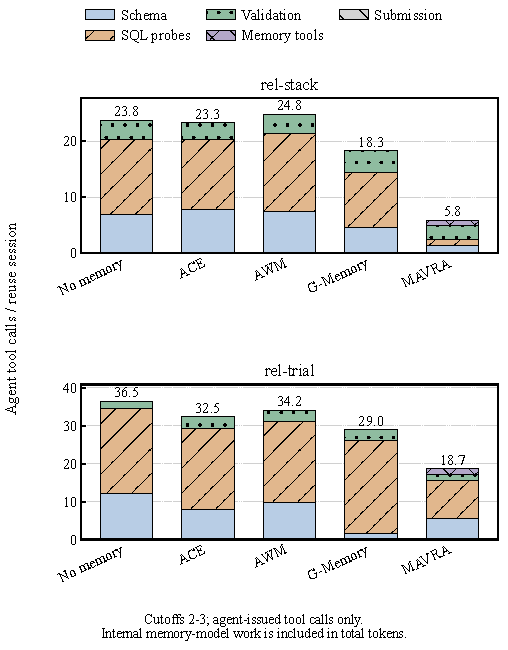
\includegraphics[width=\linewidth]{figures/reuse-work}
\fi
\caption{\bt{Mean agent tool calls per reuse session at cutoffs 2--3: six sessions per method and database, including failures.}{截点 2--3 的每个复用会话平均智能体工具调用数：每种方法、每个数据库六个会话，含失败。}}
\label{fig:reuse-work}
\Description{Two vertically stacked panels, one per database, compare all five methods. Stacked bars distinguish schema inspection, SQL probes, validation, memory tools, and submission with colors and hatching. The y-axis counts agent-issued tool calls per reuse session and starts at zero.}
\end{figure}

\bi{\emph{Tool use.} The official-API cohort compares no memory, ACE, AWM, G-Memory, and \system{} over three cutoffs (90 sessions), separately from the five-cutoff cohort. Reuse first validates prior task SQL, then retrieves definitions, skipping extraction for unchanged, freshly audited published SQL. Figure~\ref{fig:reuse-work} includes failures: \system{} makes \OfStackExplore/\OfTrialExplore{} exploration calls per reuse session versus \OfStackNoneExplore/\OfTrialNoneExplore{} without memory, retaining \OfStackValidate/\OfTrialValidate{} validations. Total-token savings are \OfStackSaveAll\%/\OfTrialSaveAll\%. Five of six task means meet the quality margin; study-adverse MAE rises \OfAdverseRegression\%, and only one of three site-success attempts is valid.}
{\emph{工具调用。}官方 API 批次在三截点比较无记忆、ACE、AWM、G-Memory 与 \system{}（90 会话），与五截点批次分别报告。复用先验证先前任务 SQL，再检索定义；未变且重新通过审计的已发布 SQL 跳过提炼。图~\ref{fig:reuse-work}计入失败：\system{} 每复用会话探索 \OfStackExplore／\OfTrialExplore{} 次，无记忆为 \OfStackNoneExplore／\OfTrialNoneExplore{} 次，并保留 \OfStackValidate／\OfTrialValidate{} 次验证。总 token 减少 \OfStackSaveAll\%／\OfTrialSaveAll\%；六项任务中五项达到质量门槛，study-adverse MAE 上升 \OfAdverseRegression\%，三次 site-success 仅一次有效。}
\bi{\emph{Reuse source.} Nine of twelve reuse sessions first validate task SQL and six keep it verbatim; none directly validates unchanged definition-compiled SQL. Explicit \code{compose\_features} calls are absent, although lookup compiles internally. At cutoff 1, the temporal audit rejects three transferred post-related features on user-engagement before a rewrite passes. These traces establish reduced exploration, with cross-task audits still required.}
{\emph{复用来源。}十二个复用会话中九个先验证任务 SQL、六个原样保留，没有直接验证原样定义编译 SQL 的会话。查找工具内部编译，但无显式 \code{compose\_features} 调用。首截点的时间审计拒绝 user-engagement 上三个迁移的帖子相关特征，改写后通过。探索减少，跨任务审计仍然必要。}
\subsection{\bt{Population sharing and maintenance}{群体共享与维护}}
\label{sec:population-eval}
\begin{table}[t]
\caption{\bt{What one question costs once the metrics are learned: the second half of the \PpAgents\ agents on TPC-DS, means over \PpRuns\ runs. Tokens include extraction; database time is part of agent time.}{指标学会之后一道题的代价：TPC-DS 上 \PpAgents\ 个智能体中的后一半，\PpRuns\ 次运行的均值。token 包括提取；数据库时间包含在智能体时间之内。}}
\label{tab:popcost}
\footnotesize
\setlength{\tabcolsep}{3pt}
\begin{tabularx}{\linewidth}{@{}Lrrrrrr@{}}
\toprule
& \bt{Turns}{轮数} & \bt{Tools}{工具} & \bt{Tokens}{token} & \bt{Time}{时间} & \bt{DB}{数据库} & \bt{Correct}{正确}\\
\midrule
\bt{No memory}{无记忆} & \PpNoneLateSteps & \PpNoneLateTools & \PpNoneLateTokK\,k & \PpNoneLateS\,s & \PpNoneLateDbS\,s & \PpNoneLateAcc\%\\
\bt{Single-agent memory}{单智能体记忆} & \PpPrivateLateSteps & \PpPrivateLateTools & \PpPrivateLateTokK\,k & \PpPrivateLateS\,s & \PpPrivateLateDbS\,s & \PpPrivateLateAcc\%\\
\bt{Example retrieval}{示例检索} & \PpTrajLateSteps & \PpTrajLateTools & \PpTrajLateTokK\,k & \PpTrajLateS\,s & \PpTrajLateDbS\,s & \PpTrajLateAcc\%\\
\bt{\textbf{\system\ (ours)}}{\textbf{\system（本文）}} & \textbf{\PpMavraLateSteps} & \textbf{\PpMavraLateTools} & \textbf{\PpMavraLateTokK\,k} & \textbf{\PpMavraLateS\,s} & \textbf{\PpMavraLateDbS\,s} & \textbf{\PpMavraLateAcc\%}\\
\midrule
\bt{\system\ vs.\ no memory}{\system\ 对无记忆} & & & \PpMavraLateTokXNone$\times$ & \PpMavraLateSpeedupNone$\times$ & & \\
\bottomrule
\end{tabularx}
\end{table}

\bi{\PpAgents{} sequential TPC-DS agents each draw seven of 35 questions, matched across methods within five paired runs (2,240 sessions). Memory starts empty. Definitions, metadata, joins, and caches are retained per question without memory, per agent with private memory, or globally with \system{}; all three share learning and maintenance mechanisms. Example retrieval shares successful questions, SQL, and derivations without maintenance. Other held-out/change studies share base metadata and caches even without memory to isolate definition reuse.}
{\PpAgents{} 个 TPC-DS 智能体依次各抽 35 题中的七题，五轮配对运行中各方法抽题一致（2,240 会话）。记忆初始为空。定义、元数据、连接和缓存分别按题（无记忆）、按智能体（私有记忆）或全局（\system{}）保留，三者共用学习维护机制。示例检索共享成功题目、SQL 与推导，但不维护。其他留出／变化实验连无记忆也共享基础元数据及缓存，以分离定义复用。}
\bi{Shared \system{} uses \PpMavraTotalTokM\,M tokens, \PpMavraTokSaveNone\% below no memory, with \PpMavraAcc\% versus \PpNoneAcc\% accuracy. It performs \PpMavraLearns{} extractions per run and reuses definitions in \PpMavraReused\% of questions; private memory performs \PpPrivateLearns{} extractions, reuses \PpPrivateReused\%, and costs \PpPrivateTotalTokM\,M tokens. Shared memory saves \PpMavraTokSavePrivate\% versus private memory. Example retrieval costs \PpTrajTotalTokM\,M with \PpTrajAcc\% accuracy. Table~\ref{tab:popcost} reports steady-state per-question costs. Publication replay and calculation checks reject \PubReplayRefused{} and \PubChainRefused{} erroneous candidates across \PubAllJudged{} verified sessions.}
{共享 \system{} 使用 \PpMavraTotalTokM\,M token，比无记忆少 \PpMavraTokSaveNone\%，正确率为 \PpMavraAcc\% 对 \PpNoneAcc\%。每轮提炼 \PpMavraLearns{} 次、\PpMavraReused\% 的题复用定义；私有记忆提炼 \PpPrivateLearns{} 次、复用 \PpPrivateReused\%、消耗 \PpPrivateTotalTokM\,M token。共享比私有少用 \PpMavraTokSavePrivate\% token；示例检索使用 \PpTrajTotalTokM\,M、正确率 \PpTrajAcc\%。表~\ref{tab:popcost}报告稳定阶段每题代价。\PubAllJudged{} 个已核实会话中，发布重放与算式检查分别拒绝 \PubReplayRefused{} 和 \PubChainRefused{} 个错误候选。}
\label{sec:cost}
\label{sec:opt-eval}
\bi{\emph{Maintenance and optimization.} After the population restatement, repairing each definition once uses \PpMavraMaintS\,s of database time versus \PpPrivateMaintS\,s for private copies. Non-breaking updates and repairs cost \AmMaintBenignS/\AmMaintRepairS\,s end to end; discarding knowledge on every write costs \ScenRelearnTok\,M relearning tokens. On one-million-row retail, \OptPublished{} of \OptDefs{} definitions receive equivalent key-range rewrites, saving \OptSaveMin--\OptSaveMax\% query time (mean \OptSaveMean\%); each paired mean-difference 95\% interval is below zero. Rewrites match \OptPeriods{} periods and are adopted by \OptHoldAdopted/\OptHoldTasks{} held-out queries. In a separate four-definition test, date re-keying invalidates every rewrite; fallback takes at most \PbFallbackMsMax\,ms and all \PbAnswers{} subsequent answers are correct (stale rewrites err by up to \PbStaleErrMax\%).}
{\emph{维护与优化。}群体更正后，每个定义修复一次使用 \PpMavraMaintS\,s 数据库时间，私有副本需 \PpPrivateMaintS\,s；正常更新／修复的端到端开销为 \AmMaintBenignS／\AmMaintRepairS\,s，每写即丢弃需 \ScenRelearnTok\,M token 重学。百万行零售中，\OptDefs{} 个定义中的 \OptPublished{} 个获得等价键区间改写，查询时间减少 \OptSaveMin--\OptSaveMax\%（均值 \OptSaveMean\%），各配对均值差的 95\% 区间均低于零。改写匹配 \OptPeriods{} 个期间，被 \OptHoldAdopted／\OptHoldTasks{} 条留出查询采用。独立四定义测试中，日期重新编键使全部改写失效；回退不超过 \PbFallbackMsMax\,ms，随后 \PbAnswers{} 个答案均正确，过期改写最高误差 \PbStaleErrMax\%。}
\begin{figure}[t]
\centering
\ifbilingual
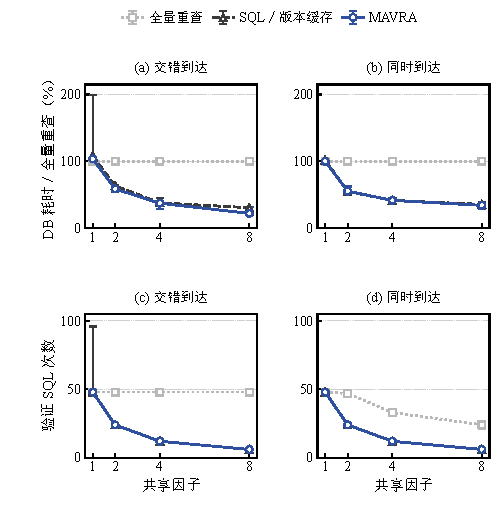
\includegraphics[width=\linewidth]{figures/fixed-sharing-zh}
\else
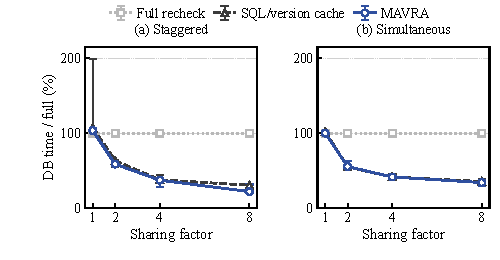
\includegraphics[width=\linewidth]{figures/fixed-sharing}
\fi
\caption{\bt{Validation time at fixed definition count, relative to matched full recheck. Points are three-block medians; error bars span all three observations.}{固定定义数下相对匹配全量重查的验证耗时。点为三轮中位数，误差棒覆盖全部三次观测。}}
\label{fig:fixed-sharing}
\Description{Two line charts compare full recheck, SQL/version cache, and MAVRA under staggered and simultaneous arrivals with a common vertical scale. Sharing factors are 1, 2, 4, and 8 definitions per table pair. The no-overlap SQL-cache outlier at about 199 percent of full-recheck database time is retained. Error bars are observed ranges, not confidence intervals. Validation query counts are reported in the text.}
\end{figure}

\bi{\emph{Shared validation.} Figure~\ref{fig:fixed-sharing} fixes 16 definitions over 16/8/4/2 active table pairs (sharing factors 1/2/4/8), eight agents and 128 requests per cell, and 100k rows per fact table. All 16 pairs receive identical warmup, benign writes and version invalidations. Three randomized blocks yield 72 cells and \MeBRequests{} valid requests. Staggered \system{} checks fall from 48 to six while full recheck stays at 48. At factor eight, matched database times are \MeBStagMavra\%/\MeBBurstMavra\% for \system{} and \MeBStagCache\%/\MeBBurstCache\% for SQL caching (staggered/simultaneous). Both reuse exact checks; full recheck also coalesces simultaneous requests. One factor-one cache run refreshes twice (96 checks; 199.36\%). Times include metadata; active tables decrease with sharing.}
{\emph{共享验证。}图~\ref{fig:fixed-sharing}固定 16 个定义，映射到 16／8／4／2 个活跃表对（共享因子 1／2／4／8），每格八智能体、128 请求，每事实表 100k 行。全部 16 表对接受相同预热、良性写入和版本失效。三轮随机顺序产生 72 格、\MeBRequests{} 次有效请求。交错到达时 \system{} 检查从 48 降至六次，整定义重查保持 48 次。因子八时，相对匹配重查的数据库耗时为 \system{} 的 \MeBStagMavra\%／\MeBBurstMavra\%、SQL 缓存的 \MeBStagCache\%／\MeBBurstCache\%（交错／同时到达）。两者复用相同检查，整定义重查也合并同时到达请求；因子一的一次缓存运行刷新两次（96 检查、199.36\% 耗时）。数据库耗时含元数据；活跃表集合随共享缩小。}
\subsection{\bt{Reuse after data changes}{数据变化后的复用}}
\label{sec:changes-eval}
\label{sec:scenarios}
\label{sec:validity}
\begin{figure}[t]
\centering
\ifbilingual
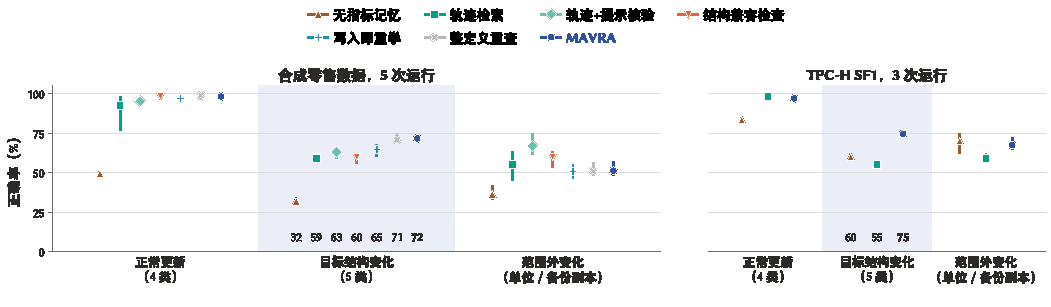
\includegraphics[width=\linewidth]{figures/two-schemas-zh}
\else
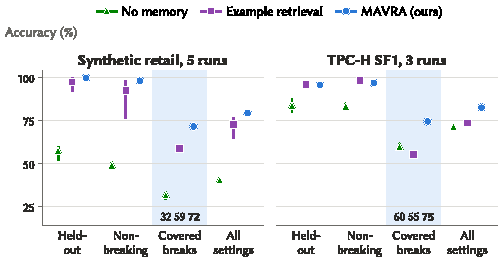
\includegraphics[width=\linewidth]{figures/two-schemas}
\fi
\caption{\bt{Accuracy over held-out questions, eleven changes and cross-agent forms (\PubScenarioScored{} answers). Equal-schema means across all \PubScenarioSettings{} settings: MAVRA \PubJointMAVRAAcc\%, AWM \PubJointAWMAcc\%. One run/method; frozen baseline controls reused.}{留出题、十一种变化及跨智能体题型的正确率（\PubScenarioScored{} 次作答）。两模式及全部 \PubScenarioSettings{} 种情形等权汇总：MAVRA \PubJointMAVRAAcc\%，AWM \PubJointAWMAcc\%。每方法一轮，复用冻结基线对照。}}
\label{fig:twoschemas}
\Description{Compact grouped bars compare ACE, AWM, G-Memory, and full MAVRA on synthetic retail and TPC-H SF1. Questions cover single periods, period differences, highest months and largest monthly increases. Groups show non-breaking updates, covered structural changes, new-agent form transfer, and all settings, on a common zero-to-100-percent scale. All settings also include the original held-out, unit and backup-source cases. Unchanged published baseline controls are reused; the repaired native method and all extra queries are freshly evaluated. Each extra question provides the same explicit business definition to a new agent. No confidence intervals or statistical-significance claim is made.}
\end{figure}

\bi{After the TPC-DS restatement (four affected questions/agent; 320 sessions/method), \system{} achieves \PpMavraChangeAcc\% accuracy at \PpMavraChangeTokK\,k tokens/question; example retrieval achieves \PpTrajChangeAcc\%/\PpTrajChangeTokK\,k and no memory \PpNoneChangeAcc\%/\PpNoneChangeTokK\,k.}
{TPC-DS 更正后每智能体重答四道受影响题（每方法 320 会话），\system{} 正确率为 \PpMavraChangeAcc\%、每题 \PpMavraChangeTokK\,k token；示例检索为 \PpTrajChangeAcc\%／\PpTrajChangeTokK\,k，无记忆为 \PpNoneChangeAcc\%／\PpNoneChangeTokK\,k。}
\bi{Equal-schema means over all \PubScenarioSettings{} settings give \system{} \PubJointMAVRAAcc\% accuracy, versus \PubJointAWMAcc\% for AWM, \PubJointACEAcc\% for ACE, and \PubJointGMemoryAcc\% for G-Memory (Figure~\ref{fig:twoschemas}). Its \PubTransferCount{} new-agent answers are all correct, matching AWM/G-Memory, with \PubTransferTokenSaving\% fewer tokens and \PubTransferCallSaving\% fewer API calls than AWM (online updates included; source learning excluded). On TPC-H, \PubTpchMAVRAAll\% trails AWM's \PubTpchAWMAll\%: append answers override correct compiled totals, and date-key/unit failures remain.}
{对两种模式及全部 \PubScenarioSettings{} 种情形等权汇总，\system{} 正确率为 \PubJointMAVRAAcc\%，AWM、ACE、G-Memory 分别为 \PubJointAWMAcc\%、\PubJointACEAcc\%、\PubJointGMemoryAcc\%（图~\ref{fig:twoschemas}）。\PubTransferCount{} 道新智能体问题全部答对，与 AWM／G-Memory 相同；比 AWM 少用 \PubTransferTokenSaving\% token 和 \PubTransferCallSaving\% API 调用（含在线更新，不含源学习）。TPC-H 的 \PubTpchMAVRAAll\% 仍低于 AWM 的 \PubTpchAWMAll\%：追加题覆盖了正确的编译结果，日期键／单位变化也仍有失败。}
\bi{Fixed-library replay covers \RsTotal{} common instances on four schemas. Correct/wrong/refused counts are \RsBenignCorrect/\RsBenignWrong/\RsBenignRefused{} for non-breaking updates, \RsStructuralCorrect/\RsStructuralWrong/\RsStructuralRefused{} for structural changes, and \RsOutsideCorrect/\RsOutsideWrong/\RsOutsideRefused{} for unit/backup changes. Of the \RsStructuralRefused{} structural refusals, \RsStructuralUnneeded{} are conservative; the remaining \the\numexpr\RsStructuralRefused-\RsStructuralUnneeded\relax{} block wrong SQL. All three errors share one TPC-H Q12 definition: a null auxiliary filter drops rows despite passing date coverage. Unit/backup failures require additional unit and source-of-record semantics.}
{固定库回放覆盖四种模式的 \RsTotal{} 个共同题次。正确／错误／拒绝数分别为：正常更新 \RsBenignCorrect／\RsBenignWrong／\RsBenignRefused{}，结构变化 \RsStructuralCorrect／\RsStructuralWrong／\RsStructuralRefused{}，单位／备份变化 \RsOutsideCorrect／\RsOutsideWrong／\RsOutsideRefused{}。\RsStructuralRefused{} 次结构拒绝中，\RsStructuralUnneeded{} 次为保守拒绝，其余 \the\numexpr\RsStructuralRefused-\RsStructuralUnneeded\relax{} 次阻止错误 SQL。三次错误来自同一 TPC-H Q12 定义：辅助过滤列为空导致丢行，但日期覆盖通过。单位／备份错误需要量纲及权威来源语义。}
\label{sec:snapshot-eval}
\bi{\emph{Snapshot binding.} A matched control fixes SQL, guards, condition cache, transactional versions, and 200k sales rows. Five counterbalanced blocks give 30 calls, excluding barrier waits from timing. Precheck releases the checked snapshot; bound execution retains it. Both serve benign writes and reject breaks before invocation; breaks after checking cause five invalid precheck results and five valid bound results. Separate version sources are used for overhead: reads average two run medians and writes use three-run medians. Precheck/bound steady-state reads take 5.1/6.9\,ms and first post-write reads 1,188/1,095.1\,ms. At 32 writers, 16 version shards retain 96.6\% of no-trigger throughput versus 36.1\% for one row.}
{\emph{快照绑定。}匹配对照固定 SQL、守卫、条件缓存、事务版本及 200k 销售行；五轮交替顺序共 30 调用，屏障等待不计时。预检查释放已核验快照，绑定执行保留它；两组均服务良性写入、拒绝调用前破坏，检查后破坏则产生五次无效预检查结果和五次有效绑定结果。开销批次的版本来源不同，读取为两轮中位数的均值、写入为三轮中位数。预检查／绑定的稳态读取为 5.1／6.9\,ms，写后首次为 1,188／1,095.1\,ms。32 写连接时，16 版本分片保留无触发器吞吐的 96.6\%，单行为 36.1\%。}
% Allow the wide evaluation figure to float while text continues.
